% Generated by support/export-artifacts.py; do not edit.
% Slug: ch54-modrm
% Source: chapters/ch54.tex:67
% TikZ source: chapters/ch54.tex:69
% Original label: \label{fig:ch54-modrm}
% Original caption (LaTeX source):
%   ModR/M fields describe the chosen opcode form, not a universal ordering of textual operands.
% Caption: ModR/M fields describe the chosen opcode form, not a universal ordering of textual operands.
% Setup: support/compiler-pseudocode.sty (TikZ libraries and shared styles).
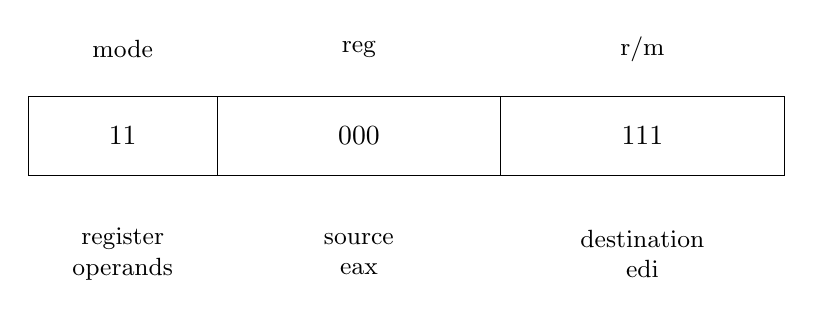
\begin{tikzpicture}[x=12mm,y=10mm]
\draw (0,0) rectangle (2,1); \draw (2,0) rectangle (5,1); \draw (5,0) rectangle (8,1);
\node at (1,0.5) {11}; \node at (3.5,0.5) {000}; \node at (6.5,0.5) {111};
\node[font=\small] at (1,1.6) {mode}; \node[font=\small] at (3.5,1.6) {reg}; \node[font=\small] at (6.5,1.6) {r/m};
\node[font=\small,align=center] at (1,-1) {register\\operands};
\node[font=\small,align=center] at (3.5,-1) {source\\eax};
\node[font=\small,align=center] at (6.5,-1) {destination\\edi};
\end{tikzpicture}

% Original figure LaTeX:
% \begin{figure}[htbp]
% \centering
% \begin{tikzpicture}[x=12mm,y=10mm]
% \draw (0,0) rectangle (2,1); \draw (2,0) rectangle (5,1); \draw (5,0) rectangle (8,1);
% \node at (1,0.5) {11}; \node at (3.5,0.5) {000}; \node at (6.5,0.5) {111};
% \node[font=\small] at (1,1.6) {mode}; \node[font=\small] at (3.5,1.6) {reg}; \node[font=\small] at (6.5,1.6) {r/m};
% \node[font=\small,align=center] at (1,-1) {register\\operands};
% \node[font=\small,align=center] at (3.5,-1) {source\\eax};
% \node[font=\small,align=center] at (6.5,-1) {destination\\edi};
% \end{tikzpicture}
% \caption{ModR/M fields describe the chosen opcode form, not a universal ordering of textual operands.}
% \label{fig:ch54-modrm}
% \end{figure}
